\subsection{Green-Funktionen für freie Teilchen}

\subsubsection*{Hamiltonoperator und Heisenberg-Gleichung}

\stp{Betrachten Teilchen mit Spin $s$; dieser wird im Folgenden nicht mitgeschrieben.}

\stp{Hamiltonoperator:}
\begin{equation}
    H = \int d^3r\,\psi^{\dagger}(\vec r,t)\left(-\frac{\hbar^2}{2m}\Delta\right)\psi(\vec r,t).
\end{equation}

\stp{Heisenberg-Bewegungsgleichung für Feldoperatoren:}
\begin{equation}
    i\hbar\,\frac{\partial}{\partial t}\psi(\vec r,t)
    = \bigl[\psi(\vec r,t),H\bigr]
    = -\frac{\hbar^2}{2m}\Delta\,\psi(\vec r,t).
\end{equation}
\qquad $\hookrightarrow \psi$ ist Operator; $\Delta$ wirkt nicht direkt auf $\psi$

\subsubsection*{Darstellung der Feldoperatoren in der Basis ebener Wellen}

Die Entwicklung des Feldoperators in Basis ebener Wellen:
\begin{equation}
    \psi(\vec r,t)=\sum_{\vec k} a_{\vec k}(t)\,\varphi_{\vec k}(\vec r).
\end{equation}
Die Einteilchenfunktionen sind ein vollständiges Orthonormalsystem und erfüllen die freie Schrödinger-Gleichung:
\begin{equation}
    \left(-\frac{\hbar^2}{2m}\Delta\right)\varphi_{\vec k}(\vec r)=E_{\vec k}\,\varphi_{\vec k}(\vec r).
\end{equation}
Für ebene Wellen gilt:
\begin{equation}
    \varphi_{\vec k}(\vec r)=\frac{1}{\sqrt{V}}\,e^{i\vec k\cdot\vec r},
    \qquad
    E_{\vec k}=\frac{\hbar^2 k^2}{2m}.
\end{equation}
Einsetzen in die Heisenberg-Gleichung liefert:
\begin{equation}
    \label{f:zeitentwOperatoren}
    \begin{aligned}
        i\hbar\,\frac{\partial}{\partial t}\sum_{\vec k} a_{\vec k}(t)\,\varphi_{\vec k}(\vec r)
         & = \sum_{\vec k} E_{\vec k}\,a_{\vec k}(t)\,\varphi_{\vec k}(\vec r),                                         \\
        \Rightarrow\quad i\hbar\,\frac{\partial}{\partial t}a_{\vec k}(t)
         & = E_{\vec k}\,a_{\vec k}(t),                                                                                 \\
        \Rightarrow\quad \underbrace{a_{\vec k}(t)}_{\text{Operator}}
         & = \underbrace{a_{\vec k}}_{\substack{\text{Operator}\\\text{zur Zeit }0}}\,e^{-\frac{i}{\hbar}E_{\vec k} t}.
    \end{aligned}
\end{equation}

\subsubsection*{Retardierte und avancierte GF}
\begin{equation}\label{f:BeginGra}
    \begin{aligned}
        G^{r,a}(1,1\mkern1mu')
         & = \pm\Theta\!\bigl(\pm(t_1-t_1\mkern1mu')\bigr)\left[G^{>}(1,1\mkern1mu')-G^{<}(1,1\mkern1mu')\right]                                                      \\
         & = \pm\Theta\!\bigl(\pm(t_1-t_1\mkern1mu')\bigr)\left(-\frac{i}{\hbar}\right)\,\erw{\psi(1)\psi^{\dagger}(1\mkern1mu')+\psi^{\dagger}(1\mkern1mu')\psi(1)}. \\
         & = \pm\Theta\!\bigl(\pm(t_1-t_1\mkern1mu')\bigr)\left(-\frac{i}{\hbar}\right)
        \sum_{\vec k,\vec k\mkern1mu'}
        \left[\erw{a_{\vec k}(t_1)a^{\dagger}_{\vec k\mkern1mu'}(t_1\mkern1mu')}+\erw{a^{\dagger}_{\vec k\mkern1mu'}(t_1\mkern1mu')a_{\vec k}(t_1)}\right]
        \frac{1}{V}e^{i(\vec k\cdot\vec r_1-i\vec k\mkern1mu'\cdot\vec r_1\mkern1mu')}
    \end{aligned}
\end{equation}

Räumlich homogenes System $\rightarrow$ es muss $G(\vec r,\vec r\mkern1mu')$ =  $G(\vec r-\vec r\mkern1mu')$ $\Rightarrow \erw{a_{\vec k}a^{\dagger}_{\vec k\mkern1mu'}}=\erw{a_{\vec k}a^{\dagger}_{\vec k}}\,\delta_{\vec k,\vec k\mkern1mu'}$\\
Sieht man in der Exponentialfunktion sehr gut. Bedeutet effektiv $\vec k = \vec k \mkern1mu'$
\begin{equation}
    G^{r,a}(1,1\mkern1mu')
    = \frac{1}{V}\sum_{\vec k}e^{i\vec k\cdot(\vec r_1-\vec r_1\mkern1mu')}
    G^{r,a}_{\vec k}(t_1,t_1\mkern1mu').
\end{equation}
mit
\begin{equation}
    G^{r,a}_{\vec k}(t_1,t_1\mkern1mu')
    = \pm\Theta\!\bigl(\pm(t_1-t_1\mkern1mu')\bigr)\left(-\frac{i}{\hbar}\right)
    \left[\erw{a_{\vec k}(t_1)a^{\dagger}_{\vec k}(t_1\mkern1mu')}+\erw{a^{\dagger}_{\vec k}(t_1\mkern1mu')a_{\vec k}(t_1)}\right].
\end{equation}

Mit der Zeitentwicklung der Operatoren (\autoref{f:zeitentwOperatoren}) folgt
\begin{equation}
    G^{r,a}_{\vec k}(t_1,t_1\mkern1mu')
    = \pm\Theta\!\bigl(\pm(t_1-t_1\mkern1mu')\bigr)\left(-\frac{i}{\hbar}\right)
    \underbrace{\erw{a_{\vec k}a^{\dagger}_{\vec k}+a^{\dagger}_{\vec k}a_{\vec k}}}_{=1\;\text{(Fermi-Antikommutator)}}
    e^{-\frac{i}{\hbar}E_{\vec k}(t_1,t_1\mkern1mu')}
\end{equation}
\begin{equation}
    \Rightarrow G^{r,a}_{\vec k}(t_1,t_1\mkern1mu') = G^{r,a}_{\vec k}(t_1-t_1\mkern1mu')
\end{equation}

Die Fourier-Transformation ähnlich wie bei der Lehman oben mit \autoref{f:FormelFürFourier}:
\begin{equation}
    \begin{aligned}
        G^{r,a}_{\vec k}(\omega) & =\int_{-\infty}^{\infty} d\tau\,e^{i\omega\tau}G^{r,a}_{\vec k}(\tau)                                                                                                               \\
                                 & = \in d\tau \frac{1}{2\pi i} \int d\omega\mkern1mu'\bigl(\mp\frac{i}{\hbar}\bigr)e^{i(\omega\pm\omega\mkern1mu'-\frac{E_{\vec k}}{\hbar})\tau} \frac{1}{\omega\mkern1mu'-i\epsilon} \\
                                 & = \mp \frac 1 \hbar \frac{1}{\mp \omega \pm \frac{E_{\vec k}}{\hbar} - i\epsilon }
    \end{aligned}
\end{equation}
liefert die Darstellung der retardierten und avancierten zeitgeordnete Gf im Frequenzraum
\begin{equation}
    G^{r}_{\vec k}(\omega)=\frac{1}{\hbar\omega-E_{\vec k}+i\varepsilon},
    \qquad
    G^{a}_{\vec k}(\omega)=\frac{1}{\hbar\omega-E_{\vec k}-i\varepsilon}.
\end{equation}

Damit liegt der Pol von $G^r_{\vec k}(\omega)$ bei der freien Einteilchenenergie $E_{\vec k}$ in der unteren Halbebene, während der entsprechende Pol von $G^a_{\vec k}(\omega)$ in der oberen Halbebene liegt. Diese analytische Struktur kodiert Kausalitaet und beschreibt im freien Fall ungedaempfte, scharf definierte Anregungen. Bei eingeschalteter Wechselwirkung wird die freie Energie in eine frequenzabhaengige, komplexe Quasiteilchenenergie $\tilde E_{\vec k}(\omega)$ umgeformt. Deren Realteil verschiebt die Lage des Pols (Energie- oder Bandenverschiebung), waehrend der Imaginaerteil eine endliche Linienbreite bzw. Daempfung erzeugt. Die Pole repraesentieren dann nicht mehr ideale freie Teilchen, sondern Quasiteilchen mit renormierter Energie und endlicher Lebensdauer.

\lend{Vorl. 20.04.2026}

\subsubsection*{Spectral Function}

Die Spektralfunktion ist durch die Differenz aus retardierter und avancierter Green-Funktion definiert:
\begin{equation}
    \hat G_{\vec k}(\omega)
    = G^r_{\vec k}(\omega)-G^a_{\vec k}(\omega)
    = 2i\,\mathrm{Im}\,G^r_{\vec k}(\omega).
\end{equation}
Mit der Dirac-Identitäet
\begin{equation}
    \frac{1}{x+i\varepsilon}=\mathcal P\frac{1}{x}-i\pi\delta(x)
\end{equation}
folgt für freie Teilchen unmittelbar
\begin{equation}
    \hat G_{\vec k}(\omega)=-2\pi i\,\delta(\hbar\omega-E_{\vec k}) = -\frac{2\pi i}{\hbar}\delta\left(\omega-\frac{E_{\vec k}}{\hbar}\right).
\end{equation}

\begin{figure}[h]
    \centering
    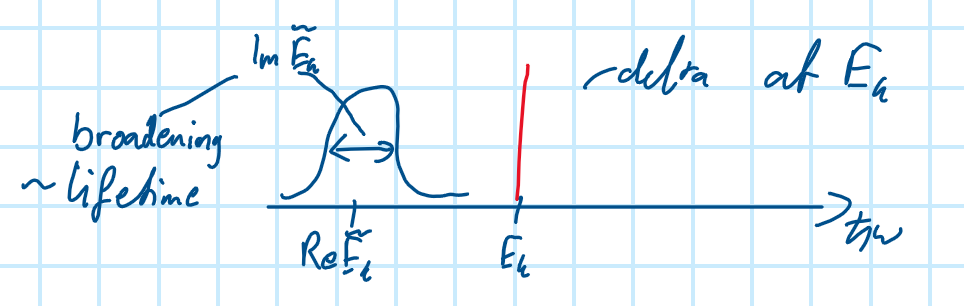
\includegraphics[width=0.78\linewidth]{Pictures/SpectralFunct.png}
    \caption{Skizze der Spektralfunktion: Im freien Fall liegt ein $\delta$-Peak bei $\hbar\omega=E_{\vec k}$ vor. Mit Wechselwirkung verschiebt sich das Maximum in Richtung $\mathrm{Re}\,\tilde E_{\vec k}$, und durch $\mathrm{Im}\,\tilde E_{\vec k}$ entsteht eine endliche Breite (Damping), die einer endlichen Lebensdauer der Quasiteilchen entspricht.}
    \label{fig:SpectralFunctionSketch}
\end{figure}

\subsubsection*{Propagators}

Für die Propagatoren gilt (analog zu \autoref{propagatoren}):
\begin{equation}
    G^{>}(1,1\mkern1mu')=-\frac{i}{\hbar}\,\langle\psi(1)\psi^{\dagger}(1\mkern1mu')\rangle,
    \qquad
    G^{<}(1,1\mkern1mu')=\frac{i}{\hbar}\,\langle\psi^{\dagger}(1\mkern1mu')\psi(1)\rangle.
\end{equation}
Analog zu der Berechnung von $G^{r,a}(1,1\mkern1mu')$ mit $a_{\vec k}(t)=a_{\vec k}e^{-\frac{i}{\hbar}E_{\vec k}t}$ (siehe Seite \pageref{f:BeginGra} und \autoref{f:zeitentwOperatoren}) folgt im Impulsraum
\begin{equation}
    G^{<}_{\vec k}(t_1,t_1\mkern1mu')
    = \frac{i}{\hbar}\,\langle a^{\dagger}_{\vec k}(t_1\mkern1mu')a_{\vec k}(t_1)\rangle
    = \frac{i}{\hbar}\,\langle a^{\dagger}_{\vec k}a_{\vec k}\rangle\,e^{-\frac{i}{\hbar}E_{\vec k}(t_1-t_1\mkern1mu')},
\end{equation}
\begin{equation}
    G^{>}_{\vec k}(t_1,t_1\mkern1mu')
    = -\frac{i}{\hbar}\,\langle a_{\vec k}(t_1)a^{\dagger}_{\vec k}(t_1\mkern1mu')\rangle
    = -\frac{i}{\hbar}\,\langle a_{\vec k}a^{\dagger}_{\vec k}\rangle\,e^{-\frac{i}{\hbar}E_{\vec k}(t_1-t_1\mkern1mu')}.
\end{equation}
Mit der Besetzungszahl $f_{\vec k}=\langle a^{\dagger}_{\vec k}a_{\vec k}\rangle$ und
$\langle a_{\vec k}a^{\dagger}_{\vec k}\rangle=1-f_{\vec k}$ erhaelt man nach Fourier-Transformation
\begin{equation}
    \begin{aligned}
        G^{\lessgtr}_{\vec k}(\omega)
         & = \int d\tau\,e^{i\omega\tau}G^{\lessgtr}_{\vec k}(\tau),
        \qquad \tau=t_1-t_1\mkern1mu',                                     \\
         & = \frac{i}{\hbar}
        \begin{Bmatrix}
            f_{\vec k} \\
            f_{\vec k}-1
        \end{Bmatrix}
        \int d\tau\,e^{i\left(\omega-\frac{E_{\vec k}}{\hbar}\right)\tau}, \\
         & = \frac{i}{\hbar}
        \begin{Bmatrix}
            f_{\vec k} \\
            f_{\vec k}-1
        \end{Bmatrix}
        \underbrace{2\pi\,\delta\!\left(\omega-\frac{E_{\vec k}}{\hbar}\right)}_{=i\hbar\,\hat G_{\vec k}(\omega)}.
    \end{aligned}
\end{equation}
und damit
\begin{equation}
    G^{<}_{\vec k}(\omega)=-f_{\vec k}\,\hat G_{\vec k}(\omega),
    \qquad
    G^{>}_{\vec k}(\omega)=(1-f_{\vec k})\,\hat G_{\vec k}(\omega).
\end{equation}

Damit enthält die Spektralfunktion die Information über die verfügbaren Zustaende, waehrend $f_{\vec k}$ deren Besetzung kodiert. Die Propagatoren $G^{<}$ und $G^{>}$ verknüpfen beide Informationen.